\intermediate{\subsection{Downloads and Installations}}

\step{Download and install \beast.}{
    \beast is available at
    \href{http://beast.bio.ed.ac.uk/Main_Page}{\url{http://beast.bio.ed.ac.uk/Main_Page}}.
    This tutorial is written for version 1.7.5 of \beast.
}

\step{Download data files from \todo{HERE}.}{
    All of the files needed for this exercise can be downloaded from \todo{HERE}.
    \begin{textbox}
        \centering
        \fbox{\begin{minipage}[c][5em][c]{0.4\textwidth}
            \begin{compactitem}
                \item data/
                \begin{compactitem}
                    \item crocodylia\_cytb.nex
                \end{compactitem}
            \end{compactitem}
        \end{minipage}}
        \caption{The files required for this tutorial.}
    \end{textbox}
}

\step{Launch BEAUTi.}{Launch BEAUTi.
    \begin{figure}
        \centering
        \fbox{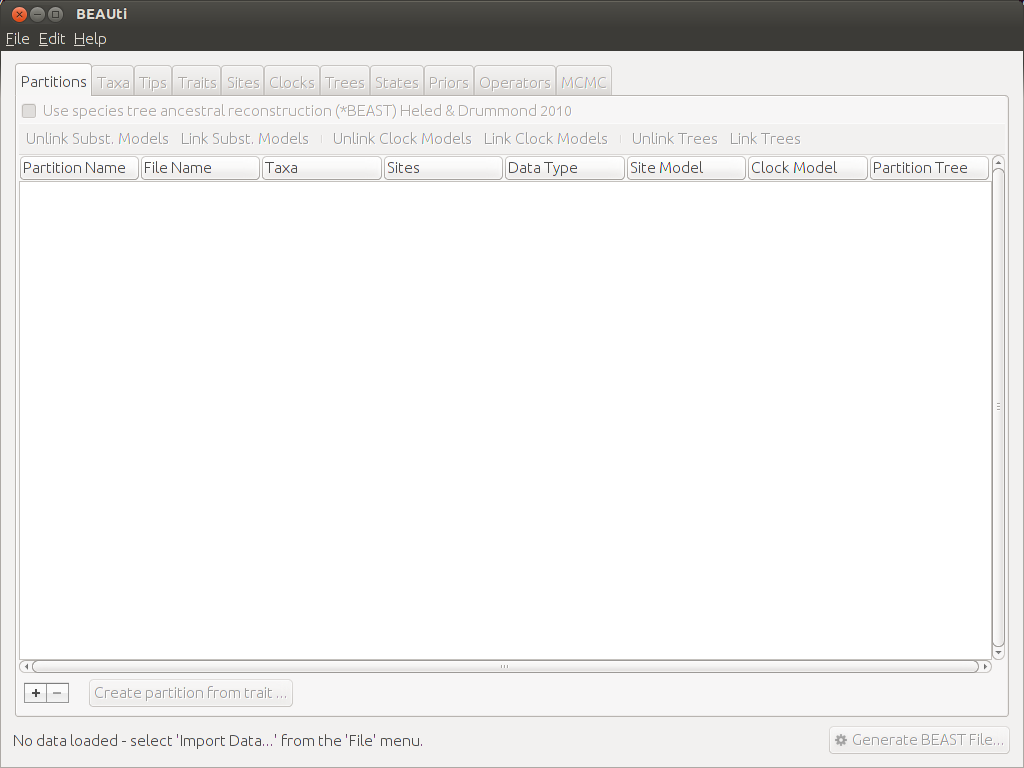
\includegraphics[width=0.6\textwidth]{../screenshots/beauti-init.png}}
        \caption{BEAUTi window}
        \label{fig:beautiInit}
    \end{figure}
}

